\documentclass[10pt]{article}
\usepackage{caption}
\usepackage{graphicx}
\graphicspath{ {./images/} }
\usepackage{fancyhdr}
\usepackage[style=british]{csquotes}
\usepackage[font={sf,it}]{caption}

%opening
\title{Microscopic Examination of Moth Specimens}
\author{  \copyright ~  {Dr. Paul J. Palmer} and {Pete Leonard}}



\pagestyle{fancy}
\makeatletter
\let\runauthor\@author
\let\runtitle\@title
\makeatother
\chead{\runtitle}
\lfoot{\runauthor}
\rfoot{\today}





\begin{document}

%\maketitle
\pagenumbering{gobble}
%\begin{abstract}
%
%\end{abstract}

Sometimes referred to as \enquote{gen dets} microscopic examination of moth specimens is a useful method of trying to identify difficult species. We are offering this service to moth recorders in VC55 and we are also happy to support those wishing to learn what they can achieve on their own.   

	\item[Get in touch] Firstly, please get in touch with Paul Palmer (\texttt{palmerpjp@gmail.com}) or Pete Leonard (\texttt{peteleonard72@gmail.com}) if  you are considering sending  any moth specimens to us so we can discuss details and check we have capacity to accept your specimens. 

	\item[General notes on specimen preparation] ID often requires examination of both external and internal features so the whole specimen should be preserved in as near perfect condition as possible. Dissection of the genitalia requires removal of the abdomen and separation of the reproductive organs and their arrangement on a microscope slide. This is only possible if the specimen is completely dessicated since the presence of any moisture will result in decay and the growth of moulds obscuring the features required for ID. Traditionally specimens were set on pins in a perfectly dehydrated state ready for examination. Specimen details were included  with labels mounted on the same pin. This is still the best method, but not many recorders are able to prepare specimens in this manner. Below are instructions for a simpler method that we consider to be the easiest way to ensure a good result. 
	
\begin{center}
	\centering
	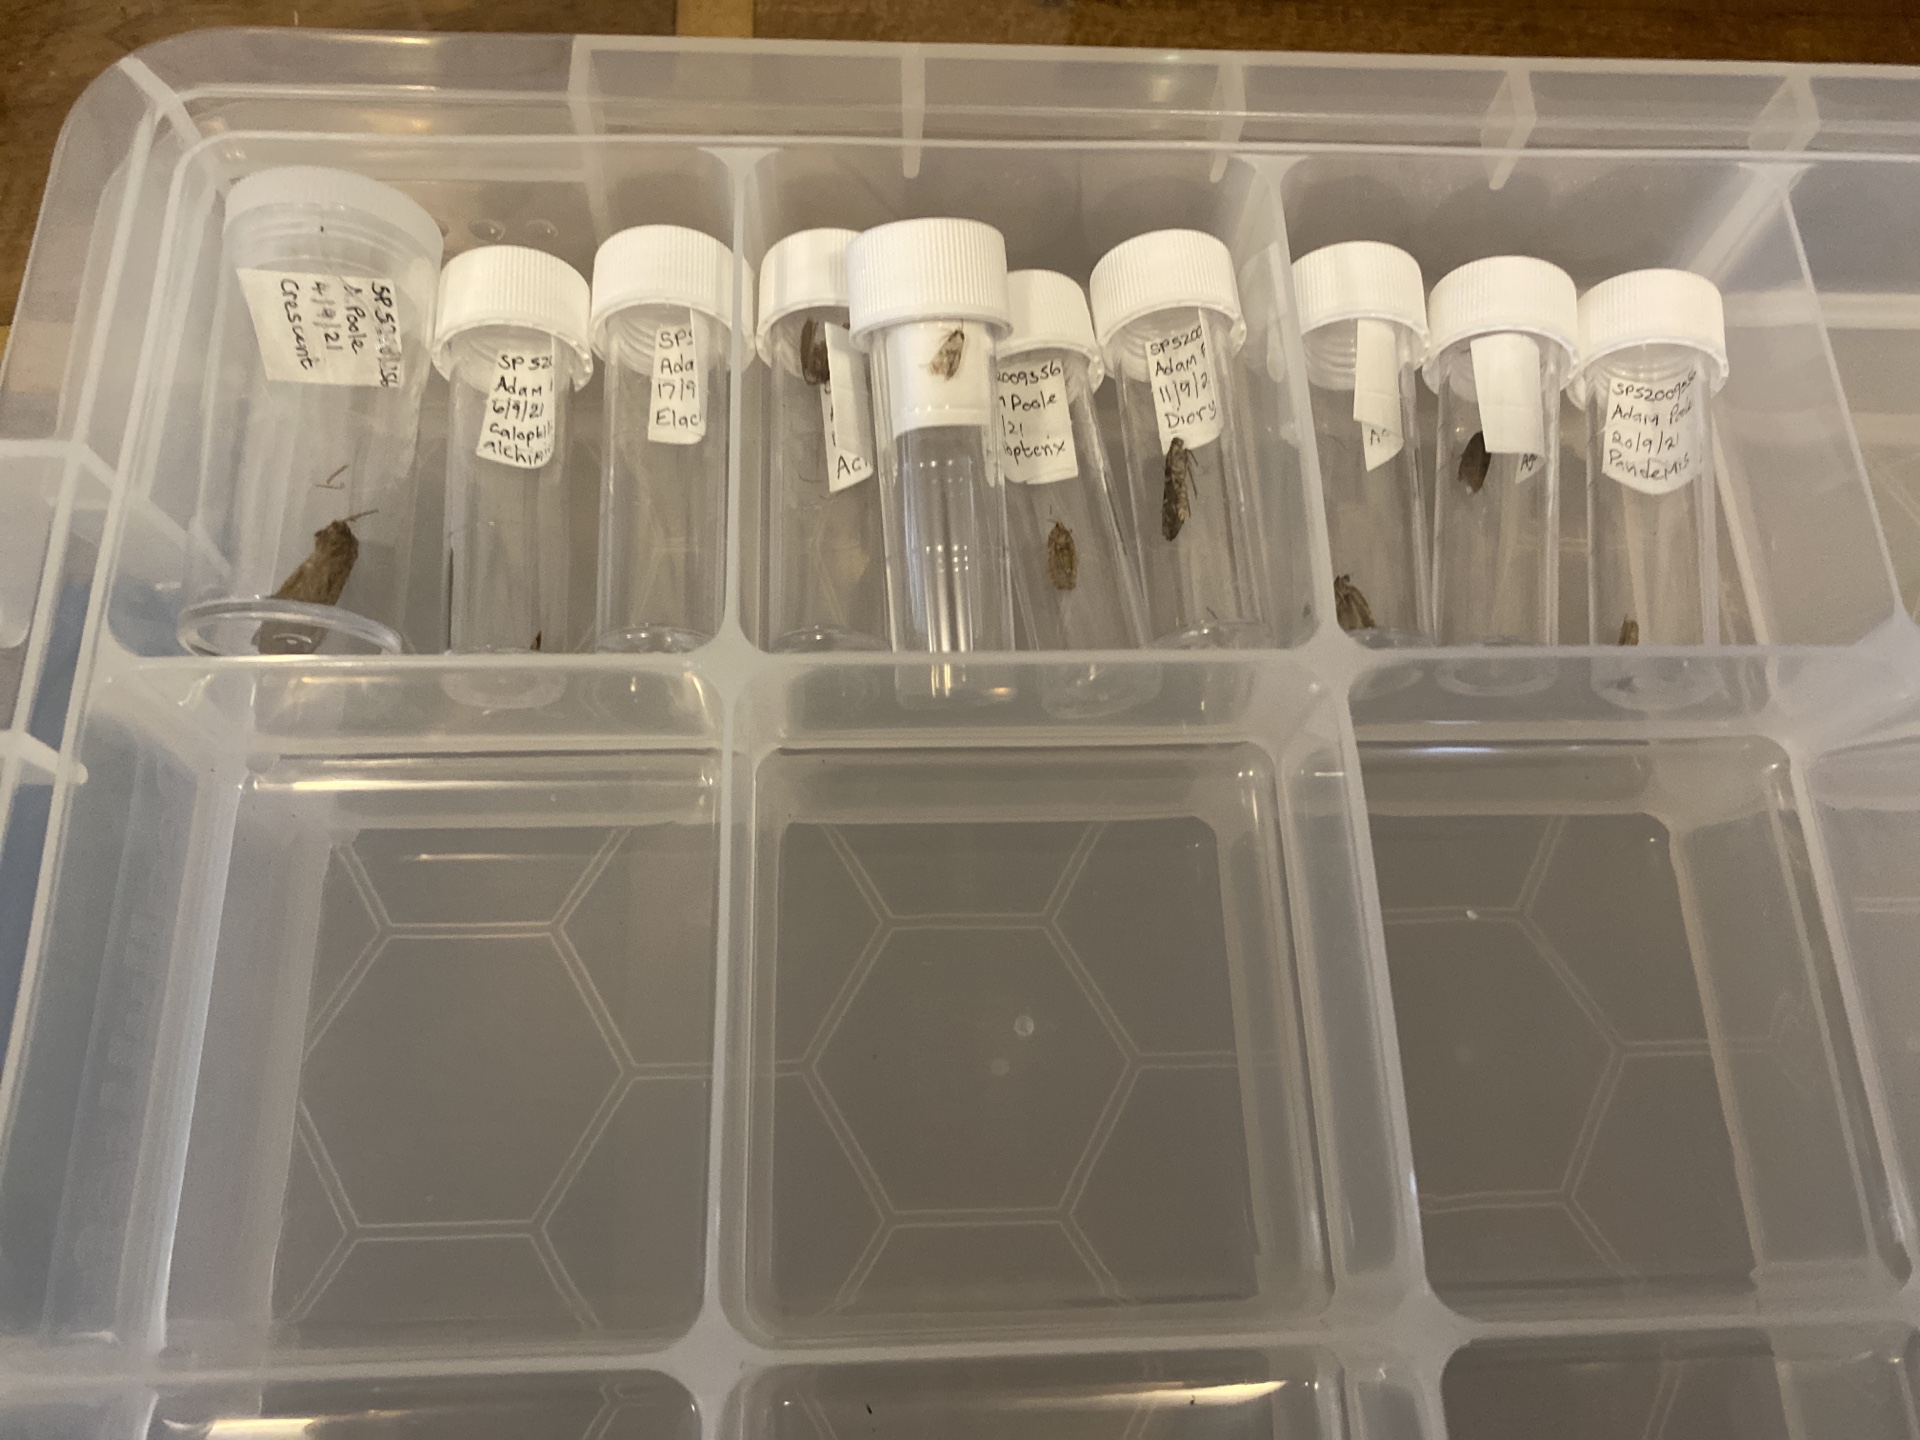
\includegraphics[width=0.3\linewidth]{images/specimens}\hfill
	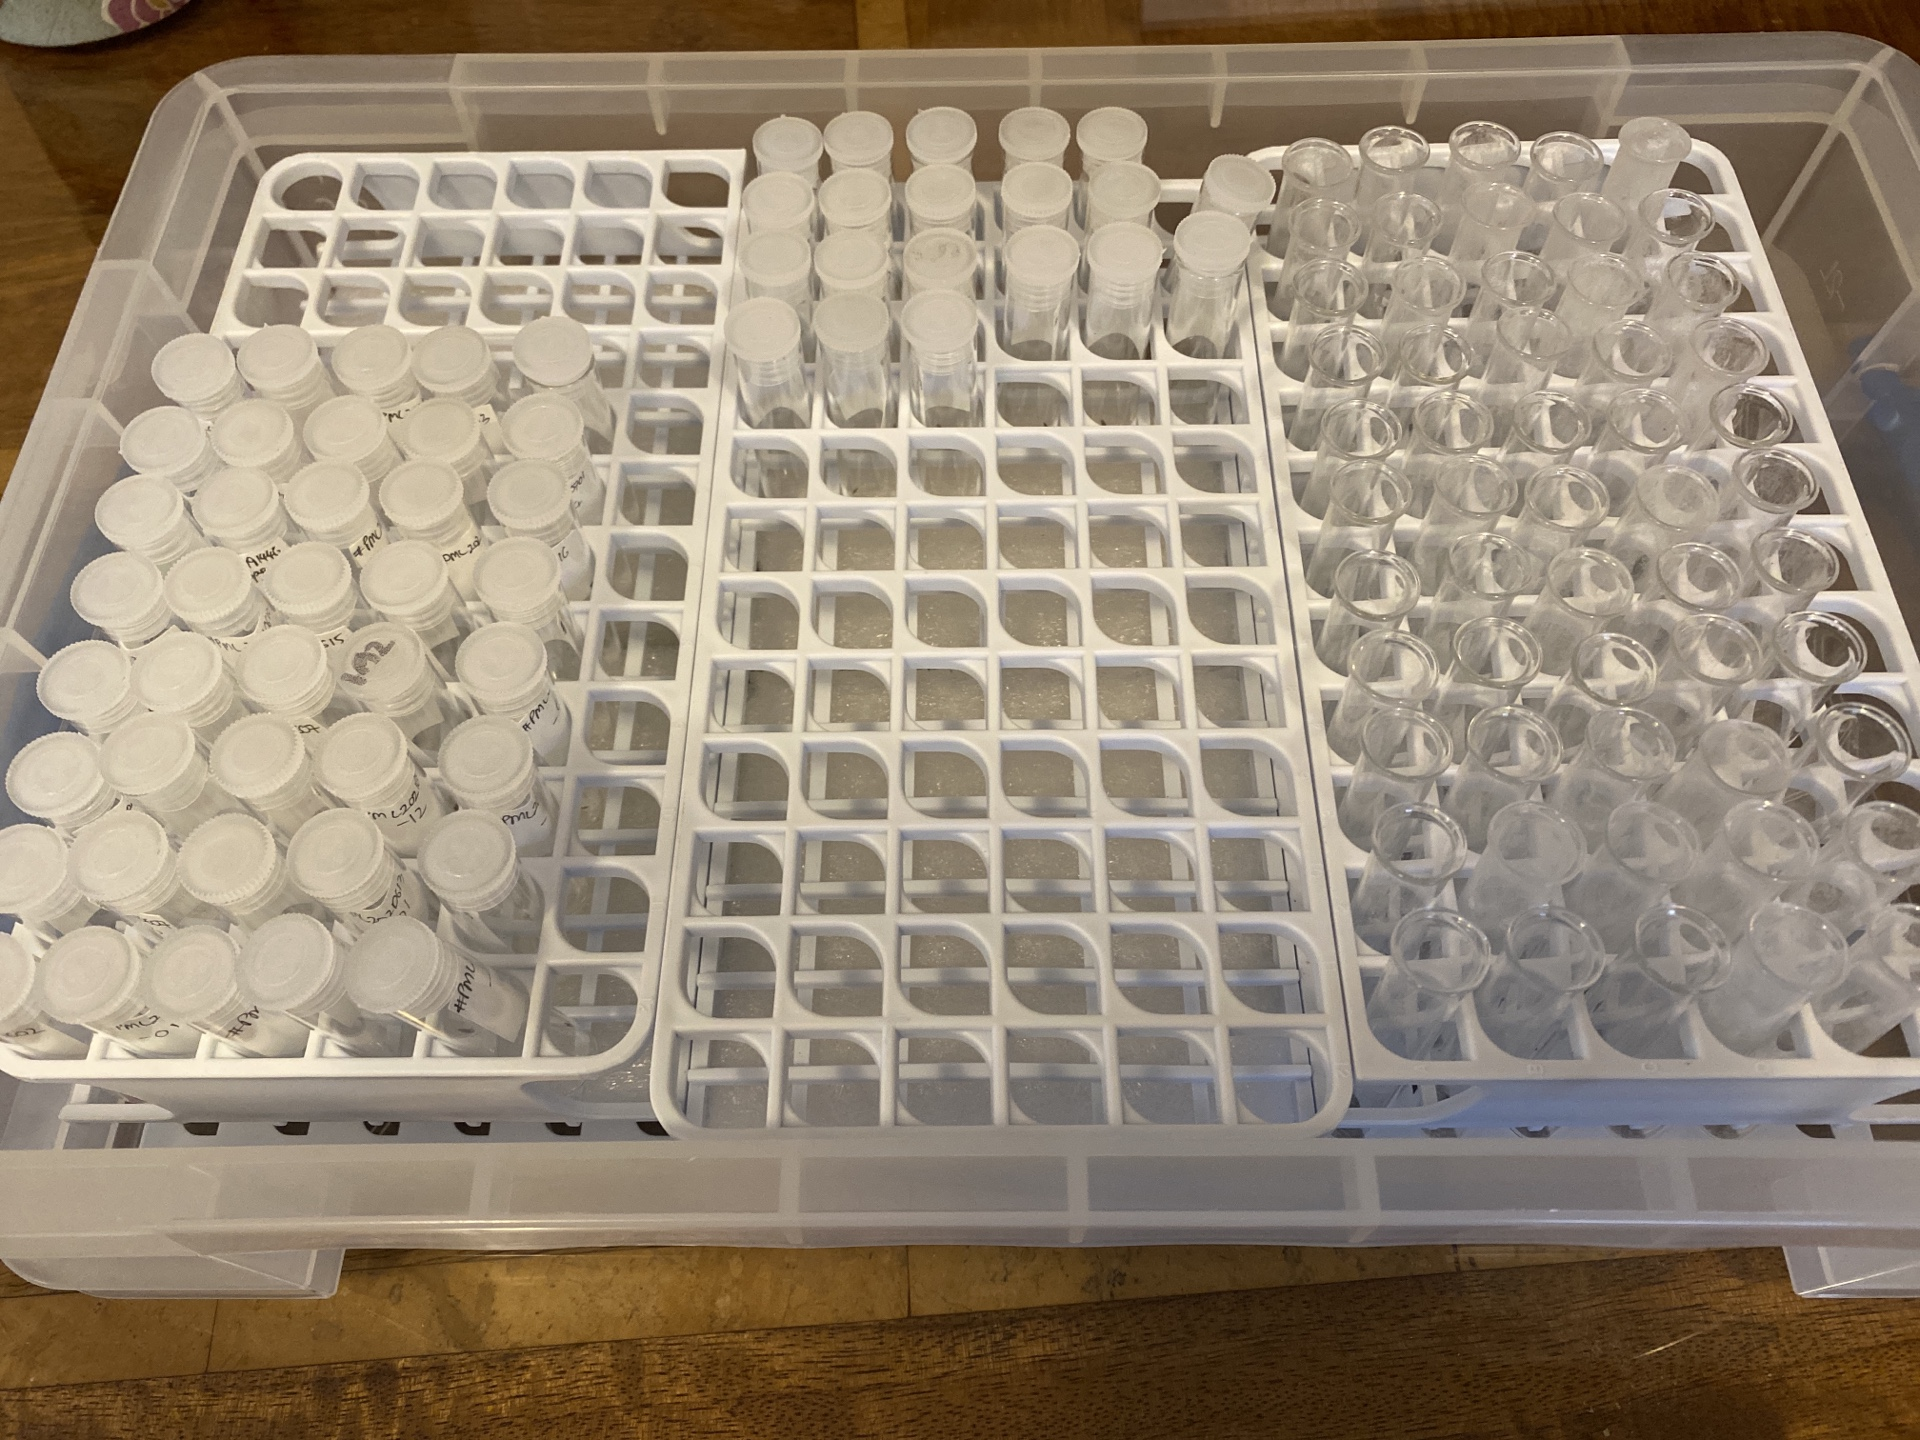
\includegraphics[width=.3\textwidth]{images/prepared}\hfill
	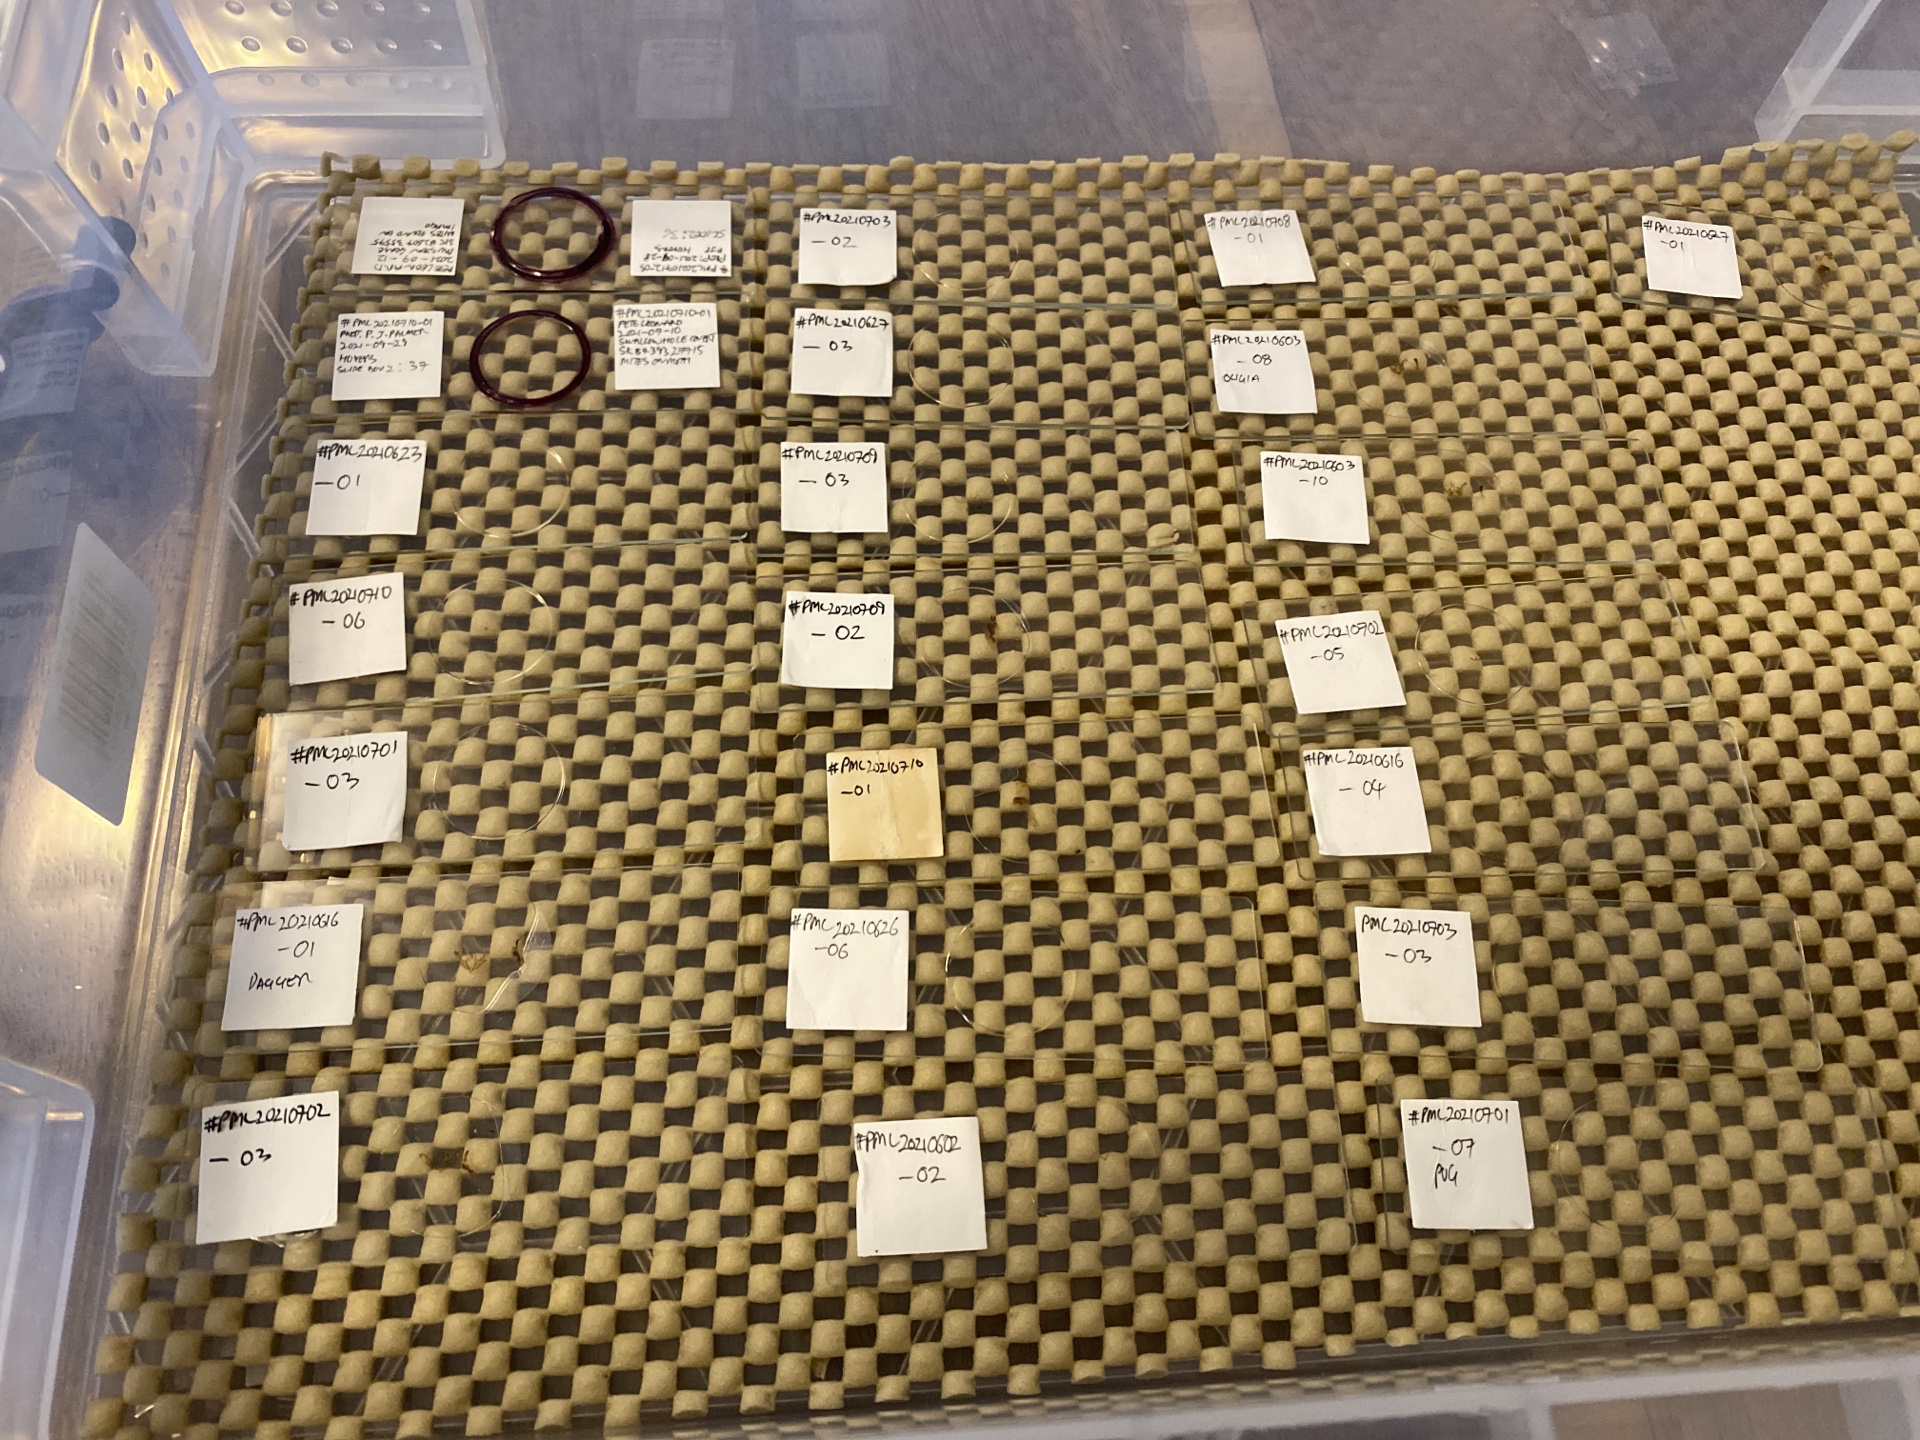
\includegraphics[width=.3\textwidth]{images/slides}\hfill
	\captionof{figure}{From left to right: Specimens as received for examination; Once photographed and catalogued each specimen is placed in a standard tube along with its label; After dissection, the label is glued to the microscope slide.}
	\label{InternalLabel}
\end{center}

Unmounted specimens should be stored singly in suitable tubes and treated in the following way:
\begin{description}

	\item[Label] Create a unique reference number for each specimen. Our suggested format is: your initials, followed by the international date (reverse date) YYYYMMDD, a hyphen, then finally a number for that day (in case there are multiple specimens taken in a day). So the third specimen taken by Paul J. Palmer on 30 April 2022 would become: PJP20220430-03. A label with this number on it should be placed inside the tube along with a single specimen. Use a pigment pen or graphite pencil. Figure~\ref{InternalLabel} illustrates how labels are used and why they must be inside the specimen tube. Without good labelling, specimens swiftly become useless. 
	\item[Data] Please complete our simple data spreadsheet, available on request. You need to complete one row per specimen with details such as locality, date and collection method. 
	\item[Photographs] If you are able to take a photograph of the live moth, in a tube if necessary, it can be a very useful aid in the identification process. Please use the unique reference number as the photograph filename.
	\item[Freezer] A minimum of 48 hours in a domestic freezer will ensure that the specimen is dead along with any mites that may be present. There is no harm in exceeding this time.
	\item[Dehydration] Exposure to dry air is needed to remove all moisture. An airing cupboard is ideal. The tubes should be uncapped, stoppered with cotton wool, and left for several weeks or longer. 
	\item[Post] Once specimens have dried, the sealed tubes containing specimens and labels may be posted to: Paul Palmer, 136 Burton Road, Melton Mowbray, Leicestershire LE13 1DL. An advance note is appreciated \\ (\texttt{palmerpjp@gmail.com}) and by arrangement, callers are always welcome.
\end{description}
	\item[What?] Please understand that our capacity for this service is limited and as such, recorders need to be judicious about what they send. Battered or worn moths, for which even identification to family level is tricky, are time-consuming and unproductive. An identification is much more likely if the list of candidate species is short. Furthermore, large numbers of common aggregate species have less scientific value (but could be useful if you would like help learning how to identify them yourself). If you would like to discuss whether or not it is worth sending a specimen, you are welcome to contact us.  
	\item[When?] We would prefer to work in small batches throughout the year rather than receive a large number of specimens at the end of the year. 

Please be patient when waiting for results, as we process specimens in batches from multiple recorders which is why we have such specific instructions on labelling and preparation. We will circulate a copy of the report containing your specimens by email when we have identified everything in the batch.

We are currently not charging for this service, but we would like to suggest recorders make a proportionate donation to a local conservation charity of... ??do we suggest an amount??

% TODO: \usepackage{graphicx} required





\end{document}
